\documentclass[a4paper,11pt]{article}

% Package to make citations superscrit with brackets
%\usepackage[super,square]{natbib}

\usepackage[style=apa]{biblatex}
\addbibresource{references.bib}

% Package to change margin size
\usepackage{anysize}
\marginsize{2cm}{2cm}{1cm}{2cm}
% Package to make headers
\usepackage{fancyhdr}
\setlength{\headheight}{13.6pt} % Fix for fancyhdr warning
\renewcommand{\headrulewidth}{0pt}
% Package for highligths
\usepackage{soul}
% Colors for the references links
\usepackage[dvipsnames]{xcolor}
% Package to link references
\usepackage{hyperref}
\hypersetup{
    colorlinks=true,
    linkcolor=black,
    citecolor=CadetBlue,
    filecolor=CadetBlue,      
    urlcolor=CadetBlue,
}
% Package for lorem ipsum
\usepackage{lipsum}
% Package for multicolumn
\usepackage{multicol}
% Package for removing paragraph identations
\usepackage{parskip}
\setlength\columnsep{18pt}
% Sets abstract
\renewenvironment{abstract}
 {\par\noindent\textbf{\abstractname}\ \ignorespaces\\}
 {\par\noindent\medskip}

\usepackage{graphicx}

\usepackage{amsmath}

\usepackage{caption}

\usepackage{amssymb}

\begin{document}

\begin{titlepage}
    \pagestyle{empty}
    \begin{center}
        % Logo
        
\includegraphics[width=0.25\textwidth]{isologo-utec.png} % Adjust path/size as needed
        \vspace{1cm}

        % Title
        {\LARGE\textbf{Modelo numérico de tiempos de impulso para optimización de trayectorias en misiones de interceptación orbital}}
        \vspace{1.5cm}

        % Authors
        {\large
            \textbf{Integrantes:} \\
            Camargo, Aldo: 202020023 \\
            Casquino, Daniel: 202110056 \\
            Vargas, Gabriel: 202310129 \\
            Whitty, Emma: 202310170 \\
            Zelaya, Jerusalén: 202220361 \\
        }
        \vspace{1cm}

        % Course
        {\large
            \textbf{Curso:} Métodos Numéricos
        }
        \vspace{0.5cm}

        % Teacher
        {\large
            \textbf{Docente:} Perez Cupe, Rosulo
        }
        \vspace{0.5cm}

        % Date
        {\large
            \textbf{Fecha de presentación:} 11 de mayo de 2025
        }
        \vfill

        {\large
            Universidad de Ingeniería y Tecnología (UTEC)
        }
    \end{center}
\end{titlepage}

% Makes header
\pagestyle{fancy}
\thispagestyle{empty}
\fancyhead[R]{\textit{Universidad de Ingeniería y Tecnología --- UTEC}}
\fancyhead[L]{}
% Makes footnotes with an asterisk
\renewcommand*{\thefootnote}{\fnsymbol{footnote}}

% \begin{abstract}
%     En el contexto de exploración espacial, la planificación de las trayectorias y
cambios de dirección requieren una cantidad considerable de apoyo terrestre. En
este contexto, surge el interés por minimizar los impulsos necesarios para
interceptar objetivos. Dados una nave perseguidora y dos objetos a interceptar,
(Xia et al., 2021) plantea una solución general para interceptar a los dos
objetos con un sólo impulso. Utilizando el método de Gibbs, se logra plantear
un sistema de ecuaciones no lineales de dos variables, el cual se puede
resolver numéricamente con el Método de Newton Raphson. Este documento busca
aplicar métodos numéricos para resolver casos particulares en MATLAB, así como
analizar la convergencia y compararla con otros métodos.
% \end{abstract}
%{\color{gray}\hrule}
%\medskip
\begin{multicols}{2}
    \renewcommand{\contentsname}{Índice}
    \tableofcontents
    \section{Introducción}

La exploración espacial ha avanzado significativamente gracias al desarrollo de tecnologías
que permiten ejecutar misiones más eficientes y de bajo costo. Sin embargo, la planificación de las trayectorias
y cambios de dirección siguen requiriendo una cantidad considerable de apoyo terrestre. En este contexto, surge el interés
por minimizar la cantidad de impulsos para llegar o interceptar a objetivos, una tarea importante en el mantenimiento de satélites
y exploración interplanetaria \parencite{ZHU20162177}.

El trabajo de Xia et al. (2021) propone un método numérico para resolver el problema de intercepción de dos objetivos
con un solo impulso, permitiendo posiciones de impulso e intercepción libres, tanto en órbitas elípticas como hiperbólicas \parencite{xia2021}.
Este enfoque reduce el problema original —de seis variables— a un sistema no lineal de solo dos variables independientes,
resuelto con el método de Newton-Raphson y estimaciones iniciales obtenidas mediante \textit{porkchop plots}.
Además, se extiende a modelos perturbados por el coeficiente J2 utilizando homotopía y corrección diferencial.

Estudios complementarios, como el de Duan y Liu (2020), exploran alternativas al clásico método de porkchop plots,
proponiendo un enfoque bidimensional más eficiente para determinar ventanas de lanzamiento, lo cual puede ser útil
en la etapa de estimación inicial de trayectorias \parencite{DUAN2020965}.

Por otro lado, el uso de propulsión eléctrica en satélites pequeños, como los CubeSats, ha abierto nuevas posibilidades para
misiones autónomas más complejas. Sistemas como los \textit{electrospray thrusters} o los \textit{gridded ion thrusters} ofrecen maniobras
precisas con menos consumo de combustible, lo cual refuerza la relevancia de modelos como el propuesto por Xia et al.\@ para planificar
trayectorias de forma óptima \parencite{oreilly2021}.

De forma complementaria, Zhu y Yan (2016) presentan un esquema de maniobra con dos impulsos tangenciales
en órbitas elípticas, que enfatiza la eficiencia de combustible bajo restricciones de tiempo y geometría, lo que sustenta
la importancia de estudiar intercepciones óptimas desde un punto de vista numérico \parencite{ZHU20162177}.
    \section{Objetivos}
\subsection{Objetivo General}
Crear un modelo computacional usando métodos numéricos que nos ayuden a resolver el problema de intersección de dos objetivos con un solo impulso. Se utilizará el método de Newton-Raphson y la matriz de Jacobiana para poder resolver el sistema de ecuaciones no lineales.
\subsection{Objetivos Específicos}
\begin{itemize}
    \item Utilizar el método numérico de Newton-Raphson utilizando una matriz jacobiana analítica para poder resolver el sistema de ecuaciones no lineales que describe el problema de intersección de dos objetos en un momento orbital.
    \item Evaluar el comportamiento del modelo en distintas condiciones iniciales como posiciones y velocidades.
    \item Analizar la precisión y eficiencia del modelo, evaluando la convergencia en distintos escenarios de intercepción. Comparando los resultados con los obtenidos en el artículo de referencia.
    \item Determinar cuales son los valores óptimos de impulso y del tiempo de aplicación, permitiéndonos interceptar el objetivo, considerando la trayectoria orbital establecida.
\end{itemize}

    \section{Justificación}

Resolver el problema de intersección de dos cuerpos en movimiento
con un sólo impulso es importante porque nos permite desarrollar
soluciones eficientes ante situaciones críticas donde se cuenta
con recursos limitados.

El uso y análisis de métodos numéricos permite comparar el desempeño de las distintas
estrategias de optimización, dando lugar a posibles mejoras con la elección de distintos
métodos. Esto contribuye al desarrollo de de modelos que trabajan con más objetivos, y por
ende reducen aún más el uso de combustible.
    \section{Marco Teórico}
\subsection{Definiciones}
\begin{itemize}
    \item \textbf{Nave perseguidora}: nave que realiza los impulsos y busca interceptar a los dos objetos.
\end{itemize}

\subsection{Conceptos}
El problema de interceptación de dos objetivos con un solo
impulso es un reto fundamental en la mecánica orbital, particularmente en las
misiones espaciales que requieren la optimización de maniobras para
minimizar el uso de combustible \parencite{Battin1999}.
\subsubsection{Interceptación Orbital}
La interceptación orbital es el proceso
mediante el cual una nave espacial ajusta su trayectoria para alcanzar
un objetivo en el espacio.
\subsubsection{Two-Body Model}
El modelo de dos cuerpos es un modelo simplificado en mecánica orbital
que describe el movimiento (elíptico) de dos cuerpos bajo la influencia
mutua de la gravedad, sin tener en cuenta otras fuerzas externas (como las
perturbaciones atmosféricas) \parencite{Cerf2013}.
\subsubsection{Impulso}
En astrodinámica, el impulso es un cambio abrupto en la
velocidad de una nave espacial, que altera su trayectoria orbital.
\subsubsection{Transferencia}
Las transferencias elípticas
son trayectorias cerradas en forma de elipse, mientras que las
transferencias hiperbólicas son trayectorias abiertas que permiten a
un objeto escapar de la atracción de un cuerpo central (como la
Tierra) \parencite{ZHU20162177}.
\subsubsection{Perturbación J2}
La perturbación J2 es el efecto causado por la
forma no esférica de la Tierra, que altera ligeramente las órbitas de
los objetos cercanos debido a la asimetría gravitacional de la Tierra
(concentrada en el ecuador).
%
\subsection{Métodos Numéricos}
\subsubsection{Gráfico Porkchop}
Este método se utiliza para visualizar las posibles combinaciones de
los tiempos de impulso $t_0$ y tiempos de intercepción $t_1$ que minimizan
el tiempo total de la misión o el uso de combustible \parencite{DUAN2020965}.

El gráfico de Porkchop calcula el coste asociado a cada combinación
de $t_0$ y $t_1$ mediante una fórmula de la forma:

\begin{equation}
    \begin{split}
        P(t_0, t_1) = \left| t_1 - t_0 - \frac{M_3(t_1) - M_3(t_0)}{n_3} \right| \\
        + \left| t_2 - t_0 - \frac{M_3(t_2) - M_3(t_0)}{n_3} \right|
    \end{split}
\end{equation}


\begin{itemize}
    \item $M_3(t)$: anomalía media en el tiempo $t$.
    \item $n_3$: movimiento medio de la órbita de la nave perseguidora.
    \item $t_2$: tiempo de intercepción con el segundo objetivo.
\end{itemize}

\begin{center}
    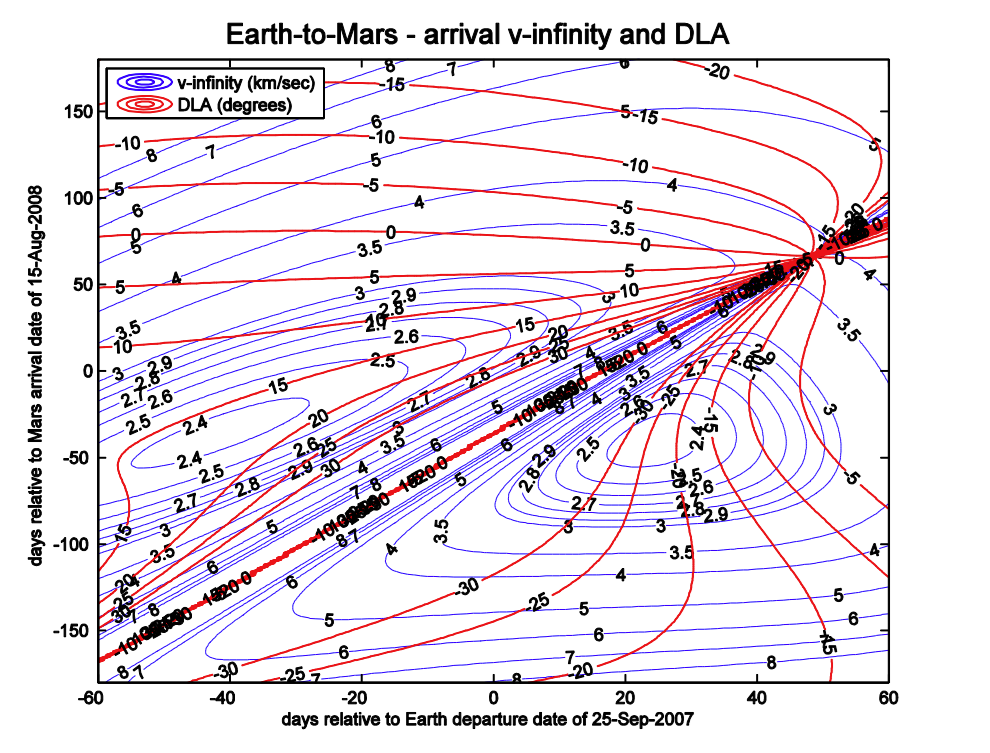
\includegraphics[width=0.4\textwidth]{porkchop_ejemplo.png}
    \captionof{figure}{Ejemplo de Porkchop plot.} \parencite{eagle2025}
\end{center}

\subsubsection{Método de Gibbs}
Una vez que se
han obtenido las estimaciones iniciales de $t_0$ y $t_1$ a partir del gráfico
Porkchop, se utiliza el Método de Gibbs para determinar la órbita
de la nave perseguidora. Gracias a esto, se reduce la cantidad de variables independientes
de seis a dos. Este concepto se explica más a profundidad en la sección de formulación del problema.

El método de Gibbs calcula la velocidad orbital de
la nave a partir de tres vectores de posición conocidos de la nave y
los dos objetivos \parencite{HE2010265}. A partir de los tres
vectores de posición $r_1$, $r_2$ y $r_3$, se calcula la velocidad de la nave
perseguidora en la órbita de intercepción con la siguiente fórmula:

\begin{equation}
    v_{3,tk} = \sqrt{\frac{\mu}{ND} \left( \frac{D \ast r_{3,tk}}{r_{3,tk}} + S \right)}
\end{equation}

Donde:
\begin{itemize}
    \item $v_{3,tk}$: vector de velocidad de la nave perseguidora en el tiempo $t_k$.
    \item $\mu$: constante gravitacional de la Tierra.
    \item N, D, y S\@: valores derivados del producto cruz entre los vectores de posición.
\end{itemize}

\subsubsection{Método de Newton-Raphson}
El Método de Newton-Raphson es un algoritmo iterativo utilizado para resolver sistemas de ecuaciones no lineales, y es esencial para refinar las soluciones obtenidas con los métodos anteriores.
En este caso, se utiliza para ajustar las variables $t_0$, $t_1$, $t_2$ y el vector de impulso $v$ hasta que se cumplan las condiciones de interceptación.

Fórmula de iteración:
\[
    x_{n+1} = x_n - J{(x_n)}^{-1} \ast F(x_n)
\]

Donde:
\begin{itemize}
    \item $x_n$ es el vector de valores actuales de las variables.
    \item $J$ es la matriz Jacobiana de las ecuaciones no lineales.
    \item $F(x_n)$ es el vector de funciones (las ecuaciones de las posiciones y tiempos de interceptación).
\end{itemize}

    \section{Formulación del problema}
El objetivo es interceptar dos objetos (naves, sálelites, etc) con un sólo impulso.
Para ello, planteamos seis variables independientes:

\begin{itemize}
    \item $t_0$: tiempo de impulso.
    \item $t_1$: tiempo de intercepción con el primer objetivo.
    \item $t_2$: tiempo de intercepción con el segundo objetivo.
    \item $\Delta{v}$: vector de impulso (contiene tres componentes).
\end{itemize}

Con el método de Gibbs, se calcula la velocidad de la nave perseguidora en los tiempos
$t_0$, $t_1$, y $t_2$. Con estos tres vectores, podemos determinar por completo la órbita
de interceptación. Luego, quedan 3 variables, en las siguientes ecuaciones:

\begin{equation}
    t_1 - t_0 = \frac{M_{3, t_1} - M_{3, t_0}}{n_3}
\end{equation}
\begin{equation}
    t_2 - t_0 = \frac{M_{3, t_2} - M_{3, t_0}}{n_3}
\end{equation}

Suponiendo que el tiempo inicial $t_i$ es conocido, y por tanto calculado $t_2$, y además despreciamos
el efecto de la perturbación J2, podemos expresar $t_2$ como una función de $t_1$ y $t_0$ \parencite{xia2021}.
Por lo tanto, el problema se reduce a dos variables independientes.

Con las ecuaciones (3) y (4), podemos armar el siguiente sistema de ecuaciones \parencite{xia2021}:

\begin{equation}
    \mathbf{F}(t_0, t_1) =
    \begin{Bmatrix}
        Q_1 \\ Q_2
    \end{Bmatrix}
    =
    \begin{Bmatrix}
        0 \\ 0
    \end{Bmatrix}
\end{equation}

donde
\begin{equation}
    \left\{
    \begin{aligned}
        Q_1 & = (t_1 - t_0) - \frac{M_{3, t_1} - M_{3, t_0}}{n_3} \\
        Q_2 & = (t_2 - t_0) - \frac{M_{3, t_2} - M_{3, t_0}}{n_3}
    \end{aligned}
    \right.
\end{equation}

Note que $t_0 < t_1 < t_2$.

Posteriormente, se estudiarán las variables $M_{j,t_k}$. Estos variables, que representan la anomalía,
media, se calculan con la ecuación de Kepler \parencite{xia2021}, y son críticas para el modelo matemático
ya que permiten calcular la posición de un objeto que se mueve en una de las tres órbitas, sobre todo la de interceptación.
\end{multicols}

\printbibliography[title={Referencias}]

\end{document}